%
% Appendix C.- About Quotes and Photos
%

\chapterimage{TuringMachine.pdf} % Chapter heading image

\chapter{About Quotes and Photos}
\label{apx:photos}

\begin{quote}
\begin{flushright}
\emph{What we know is little, \\
combined with tenacious concentration on a subject\\
and what we are ignorant of is immense.}\\
Pierre-Simon Laplace
\end{flushright}
\end{quote}
\bigskip

{\color{red} TODO: Explain why are important quotes and photos}

\subsection{Quotes}

{\color{red} Itroduce this section.}

\bigskip

\emph{Perfection is achieved not when there is nothing more to add, but when there is nothing left to take away.} Antoine de Saint-Exupéry.

{\color{red} This is a critical idea in the theory of nescience, although there are some differencies. I think Saint-Exupéry is talking more about what we have called redudancy, rather than the concept of surfeit. Moreover, Saint-Exupéry is true as long as the inaccuracy is zero.}

\bigskip

\emph{Computers are useless, they can only give you answers.} Pablo Picasso.

{\color{red} As I have said in the Preface of the book, this quote triggered everything.}

\bigskip

\emph{If presented with a choice between indifferent alternatives, then one ought to select the simplest one.} Occam’s razor principle.

{\color{red} I am sure that many people will claim that the theory of nescience is just Occam on steroids. By I think there are big differences, as I have already described in the book.}

\bigskip

\emph{Mathematics may be defined as the subject in which we never know what we are talking about, nor whether what we are saying is true.} Bertrand Russell.

{\color{red} Maybe I can talk here about Hilbert-Frege controversy, and what Russell means with this quote.}

\bigskip

\emph{Sometimes it’s the people no one imagines anything of who do the things that no one can imagine.} Alan Turing.

{\color{red} Hopefully Turing is talking about me :)}

\bigskip

\emph{Information is the resolution of uncertainty.} Claude Shannon.

{\color{red} TODO: Explain}

\bigskip

\emph{Some mathematical statements are true for no reason, they’re true by accident.} Gregory Chaitin.

{\color{red} TODO: Explain}

\bigskip

\emph{All great work is the fruit of patience and perseverance, combined with tenacious concentration on a subject over a period of months or years.} Santiago Ramón y Cajal.

{\color{red} Mention the book of Cajal.}

\bigskip

\emph{To go where you don’t know, you have to go the way you don’t know.} San Juan de la Cruz

{\color{red} TODO: Explain}

\bigskip

\emph{We are all agreed that your theory is crazy. The question which divides us is whether it is crazy enough.} Niels Bohr.

{\color{red} TODO: Explain}

\bigskip

\emph{Wanderer, there is no road, the road is made by walking.} Antonio Machado.

{\color{red} TODO: Explain}

\bigskip

\emph{A little inaccuracy sometimes saves tons of explanations.} Saki.

{\color{red} TODO: Explain}

\bigskip

\emph{Everything should be made as simple as possible, but not simpler.} Albert Einstein

{\color{red} TODO: Explain}

\bigskip

\emph{There are known knowns. These are things we know that we know. There are known unknowns. That is to say, there are things that we know we don’t know. But there are also unknown
unknowns. There are things we don’t know we don’t know.} Donald Rumsfeld.

{\color{red} TODO: Explain}

\bigskip

\emph{It is not the answer that enlightens, but the question.} Eugène Ionesco.

{\color{red} TODO: Explain}

\bigskip

\emph{Invert, always invert.} Carl Gustav Jacob Jacobi.

{\color{red} TODO: Explain}

\bigskip

\emph{Always look for tricks.} Antonio García.

{\color{red} TODO: Explain}

\bigskip

\emph{Anyone who regards games simply as games and takes work too seriously has grasped little of either.} Heinrich Heine.

{\color{red} TODO: Explain}

\bigskip

\emph{Science may be regarded as the art of data compression.} Li \& Vitányi.

{\color{red} TODO: Explain}

\bigskip

\emph{To be surprised, to wonder, is to begin to understand.} José Ortega y Gasset.

{\color{red} TODO: Explain}

\bigskip

\emph{We are to admit no more causes of natural things than such as are both true and sufficient to explain their appearances.} Isaac Newton

{\color{red} TODO: Explain}

\bigskip

\emph{What we know is little, and what we are ignorant of is immense.} Pierre-Simon Laplace

{\color{red} TODO: Explain}

\bigskip

\emph{When academics encounter a new idea that doesn’t conform to their preconceptions, there’s often a sequence of three reactions: first dismiss, then reject, and finally declare it obvious.} S. Sloman and P. Fernbach.

{\color{red} TODO: Explain}

%
% Subsection: About the Photos
%

\subsection{Photos}

In this Appendix we explain the intended meaning of the photographs included at the beginning of each chapter. All the photographs are royalty-free (or at least this is what Google Images says). Photographs have been pre-processed with GIMP\footnote {www.gimp.org}, the GNU image manipulation program: we have applied a dotify filter (Artistic filter, GIMPressionist), and then altered the color map (Colors, Colorize) with a Hue/Saturation/Lightness levels of 24/84/10.

\subsection* {The Torch Bearers}

\begin{wrapfigure}{L}{0.3\textwidth}
\centering
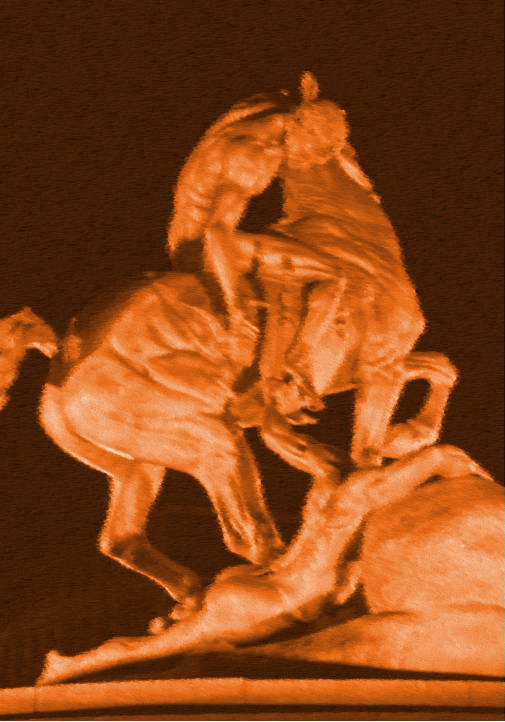
\includegraphics[width=0.15\textwidth]{Los_portadores_de_la_antorcha_-_05.pdf}
\end{wrapfigure}

The Torch Bearers is an aluminum sculpture created by the American artist Anny Hyatt Huntington, and donated to the city of Madrid in 1955. The sculpture is currently located at Universidad Complutense campus. The sculpture represents and old dying man that before to die pass the torch (a symbol of knowledge) to a young riding man that will continue the quest of perfect knowledge. The artist created other copies in bronze of the same sculpture that are located in Valencia, La Habana, and several cultural organizations around the United States.

\subsection* {Ancient Greek Philosophers}

\begin{wrapfigure}{L}{0.3\textwidth}
\centering
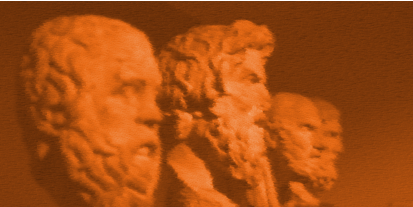
\includegraphics[width=0.30\textwidth]{Philosophers.pdf}
\end{wrapfigure}

The carved busts of Greek philosophers Socrates, Antisthenes, Chrysippus, and Epicurus, located at the British Museum in London. The ideas and achievements of the ancient Greeks philosophers changed their world and had a huge influence in Western culture. Philosophers like Socrates, Plato and Aristotle formulated the first scientific explanations about how the world worked, and they pioneer a new way of thinking, based on reason and rational thought. The scientific explanation of how the Universe works formulated by Aristotle was accepted as true during more than two thousands years.

\subsection* {Ars Magna}

\begin{wrapfigure}{L}{0.3\textwidth}
\centering
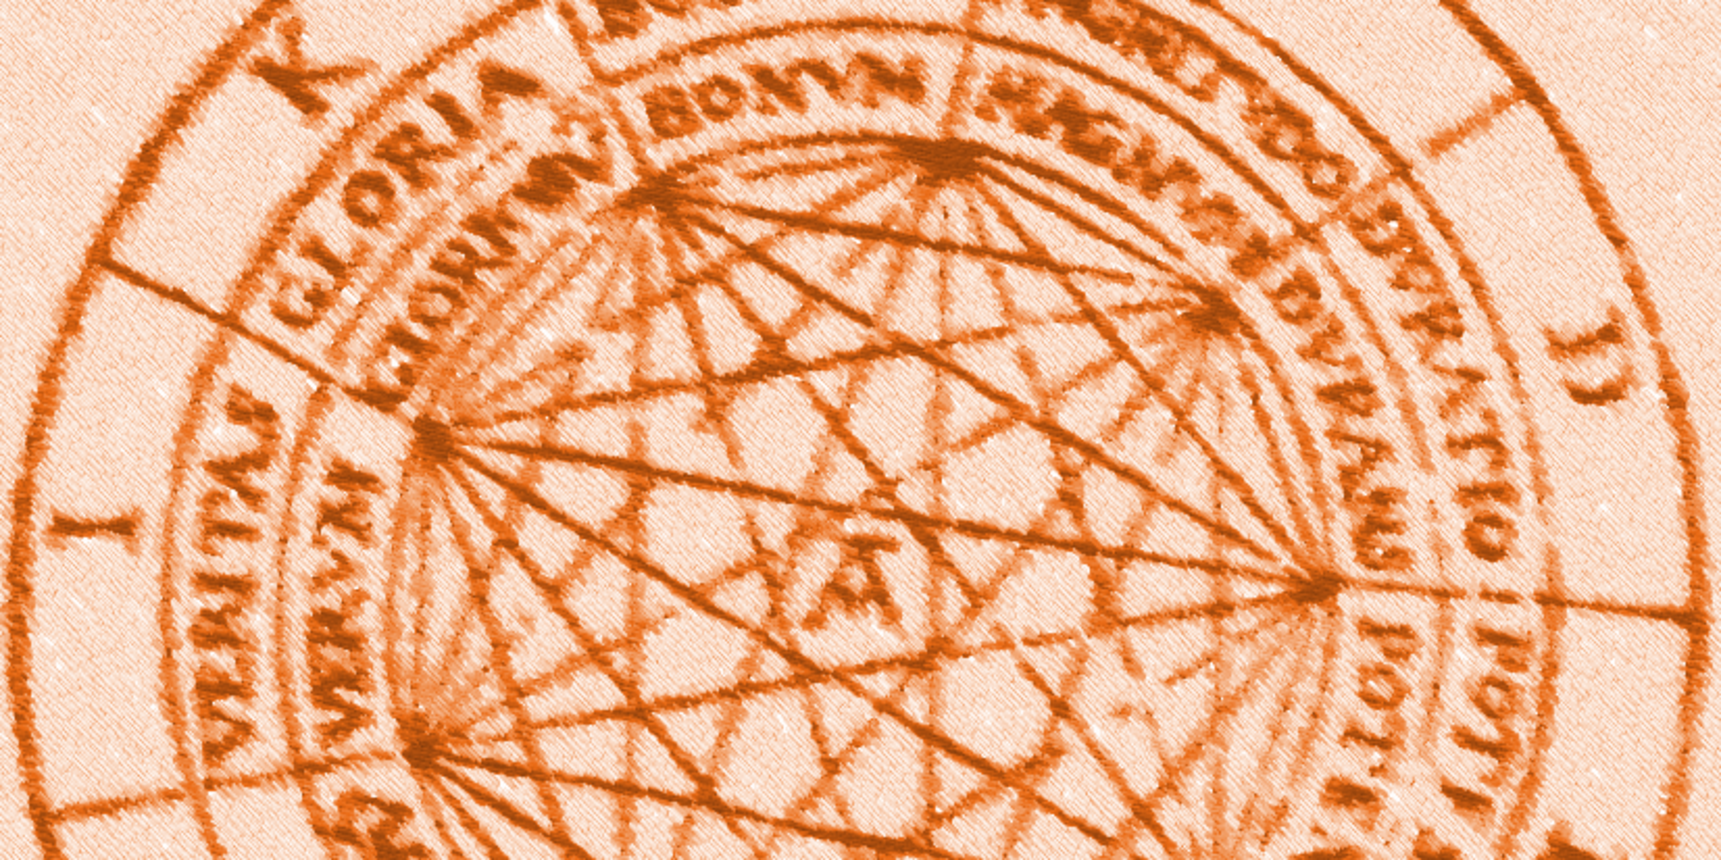
\includegraphics[width=0.30\textwidth]{Ramon_Llull_-_Ars_Magna_Fig_1.pdf}
\end{wrapfigure}

Ars Generalis Ultima or Ars Magna (The Ultimate General Art) was a book published by the Spanish philosopher Raimundo Lulio in 1305. The book contained the description of a mechanical device capable of answering any argument or question abut Christian beliefs by means of using logic and reason. The machine operated by rotating a collection of concentrically arranged circles to combine a fixed set of fundamental concepts. In this way, the device could show all possible truths about the subject of inquiry. The method was an early attempt to use logical means to produce new knowledge, and it was the inspiration for the methodology of finding interesting questions described in this book.

\subsection* {Galileo's Telescope}

\begin{wrapfigure}{L}{0.3\textwidth}
\centering
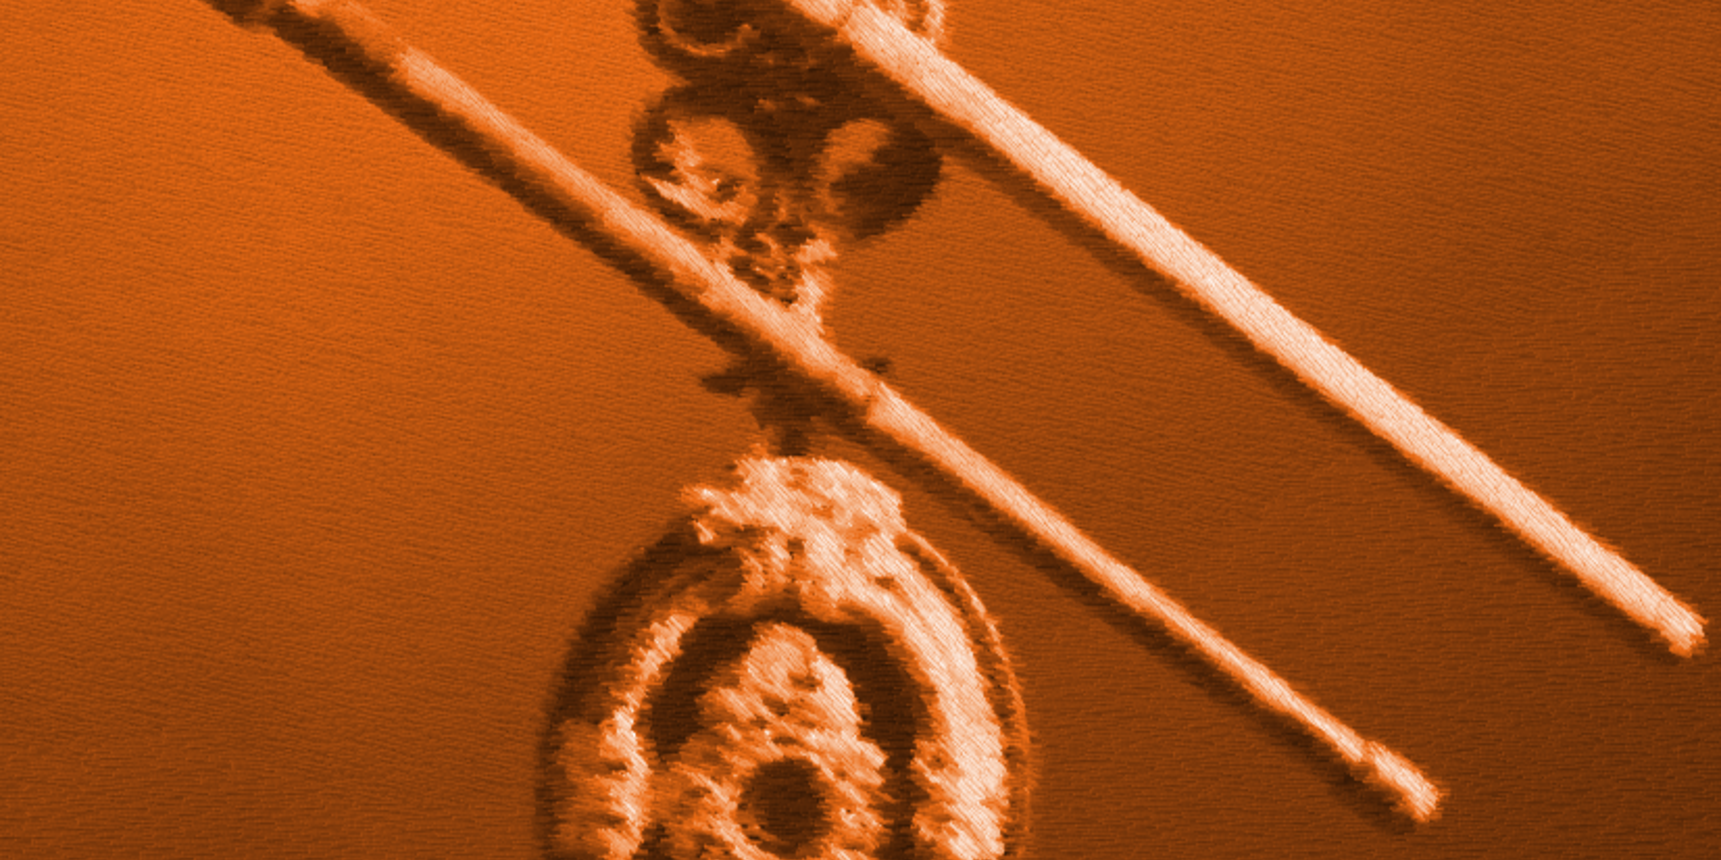
\includegraphics[width=0.30\textwidth]{Galileos-telescope-002.pdf}
\end{wrapfigure}

Galileo Galilei was an Italian astronomer, physicist, engineer, philosopher and mathematician. Galileo was the first scientist to clearly state the usefulness of mathematics to discover the laws of nature. Galileo also played a major role in the scientific revolution of the seventeenth century, introducing important innovations in the scientific method. In 1610, Galileo built a telescope and looked up at the heavens. His discoveries revolutionized the field of astronomy and changed our understanding of the Universe.

\subsection* {Königsberg Bridges}

\begin{wrapfigure}{L}{0.3\textwidth}
\centering
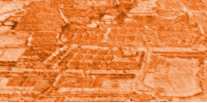
\includegraphics[width=0.30\textwidth]{Koenigsberg_Map_by_Bering_1613.pdf}
\end{wrapfigure}

The old city of Königsberg in Prussia (now Kaliningrad, Russia) was laid on both sides of the Pregel river. The city had two large islands which were connected to each other and to mainland by seven bridges. The seven bridges problem is a classical problem in mathematics that asks to devise a walk that would cross each of the seven bridges once and only once, starting and ending at any point, not necessarily the same. The Swiss mathematician Leonhard Euler proved in 1736 that the problem has no solution. The work of Euler laid the foundations of a new mathematical discipline: Graph Theory.

\subsection* {The Turing Machine}

\begin{wrapfigure}{L}{0.3\textwidth}
\centering
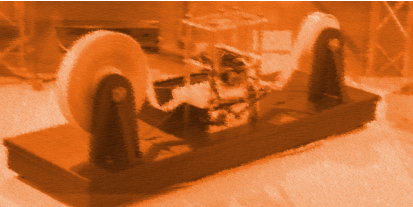
\includegraphics[width=0.30\textwidth]{TuringMachine.pdf}
\end{wrapfigure}

In 1936, the British mathematician Alan Turing proposed a formal model for a hypothetical machine and claimed that his machine could compute anything that humans could compute following an algorithm. The model was a highly convincing one, and simple enough to allow precise mathematical analysis. If fact, the model had many of the ideas that ten years later electrical engineers used to build real computers. The Turing machine was one of this few moments in the history of science in which theory preceded practice.

\newpage

\subsection* {Morse key}

\begin{wrapfigure}{L}{0.3\textwidth}
\centering
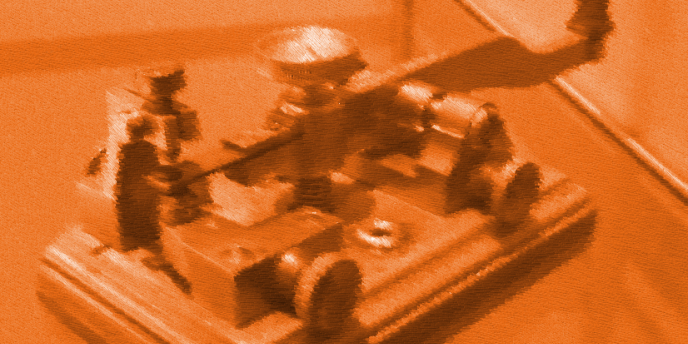
\includegraphics[width=0.30\textwidth]{Morse_key.pdf}
\end{wrapfigure}

A switching device used to send messages along a wire. The system sends pulses of electric current using the Morse code. Morse code is named after Samuel F. B. Morse, the inventor of the telegraph. The code is composed by a standardized sequence of short and long signals called \emph{dots} and \emph{dashes}, although it is not a binary code, since the code alphabet also includes symbols for the separation between letters and words. The average bit length per character for the English language is 2.53, a remarkable result, given the fact that the code was designed intuitively, without knowing any of the (later discovered) results of coding theory.

\subsection* {Mandelbrot Set}

\begin{wrapfigure}{L}{0.3\textwidth}
\centering
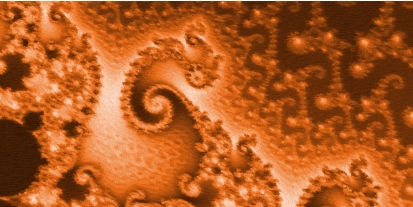
\includegraphics[width=0.30\textwidth]{Mandelbrot.pdf}
\end{wrapfigure}

The Mandelbrot set is created by sampling the complex numbers, and determining for each sample whether the result of iterating a function goes to infinity. Treating the real and imaginary parts of each number as image coordinates, pixels are colored according to how rapidly the sequence diverges, with black used for points where the sequence does not diverge. Images of the Mandelbrot set exhibit an elaborate boundary that reveals progressively ever-finer, self-similar, recursive detail at increasing magnifications. However, according to Kolmogorov complexity, the set presents a very low complexity.

\subsection* {XXX: XXX}

Xxx xxxx x xxx xx xxxxxx

\subsection* {Athena's Owl}

\begin{wrapfigure}{L}{0.3\textwidth}
\centering
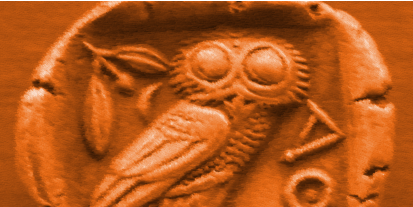
\includegraphics[width=0.30\textwidth]{owl.pdf}
\end{wrapfigure}

A silver coin depicting the owl that traditionally accompanies Athena. Athena is the virgin goddess of wisdom in Greek mythology. The owl has been used as a symbol of knowledge, wisdom, perspicacity and erudition throughout the Western world, perhaps because their ability to see in the dark. The German philosopher Hegel famously noted that "the owl of [Athena] spreads its wings only with the falling of the dusk", meaning that philosophy comes to understand a historical condition just as it passes away. In this sense, Hegel asserts that Philosophy cannot be prescriptive because it understands only in hindsight.

\subsection* {The Thinker}

\begin{wrapfigure}{L}{0.3\textwidth}
\centering
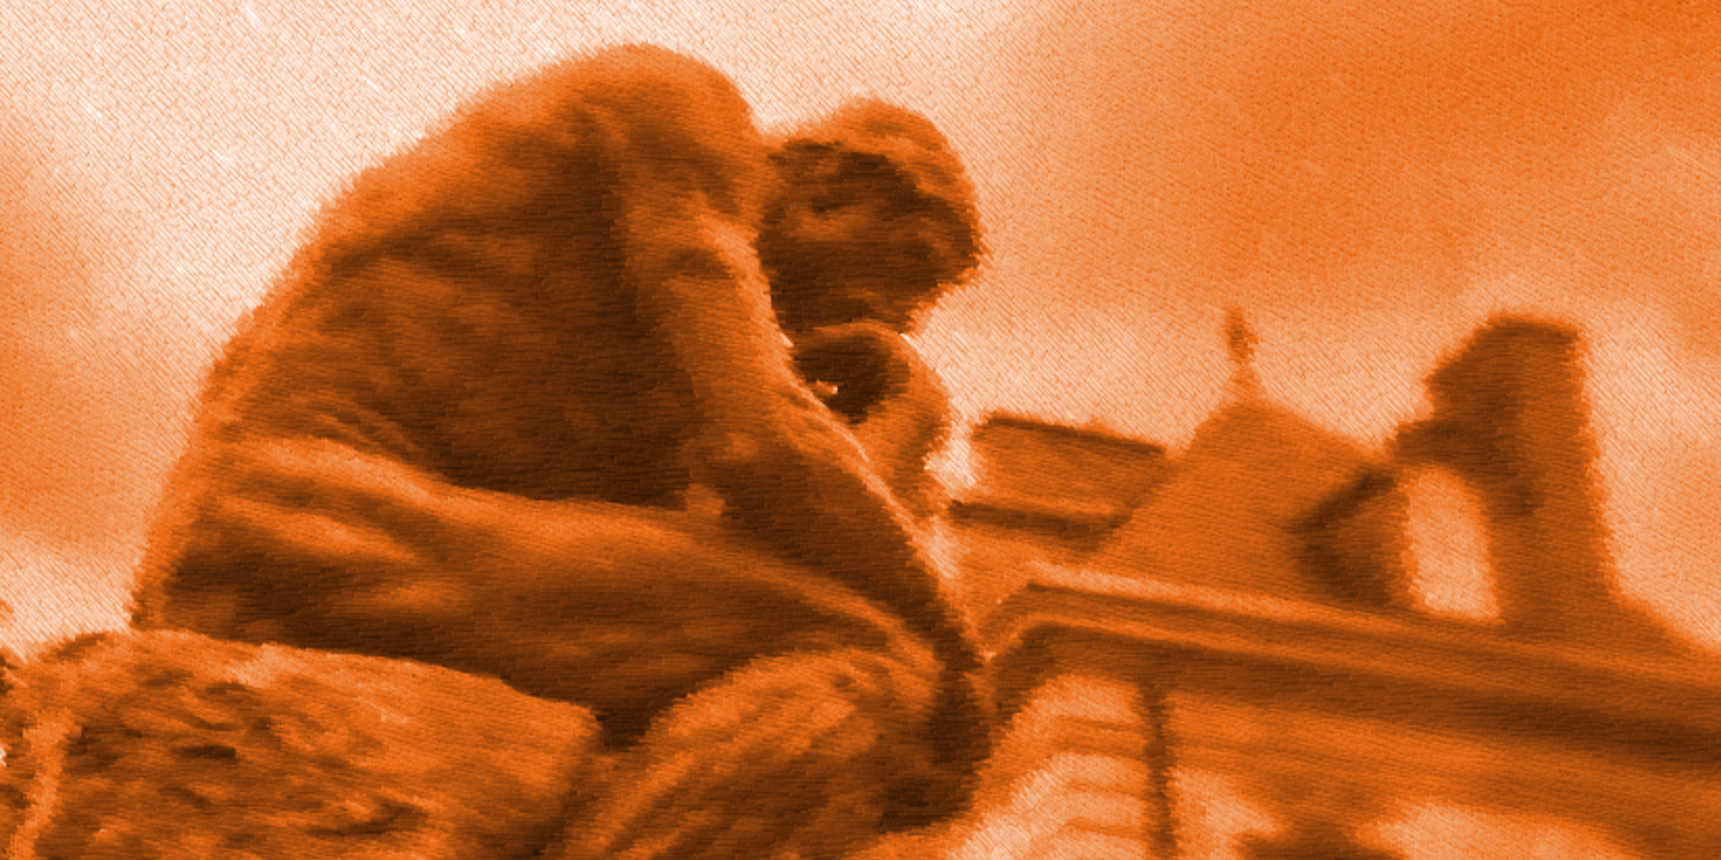
\includegraphics[width=0.30\textwidth]{thinker.pdf}
\end{wrapfigure}

The Thinker is a bronze sculpture created by the French artist Auguste Rodin. The sculpture represents a nude male figure sitting on a rock with his chin resting on one hand. Originally created as part of a larger composition (The Gates of Hell), later the artist decided to treat the figure as an independent work, and at a larger size. There are about 28 full size castings located in museums and public places all around the world (Geneva, Brussels, San Francisco, New York, Buenos Aires, etc.), and many others at different scales. A common interpretation of the sculpture is as an image of the deep thoughts required to find the right questions in philosophy.

\subsection* {R.U.R.}

\begin{wrapfigure}{L}{0.3\textwidth}
\centering
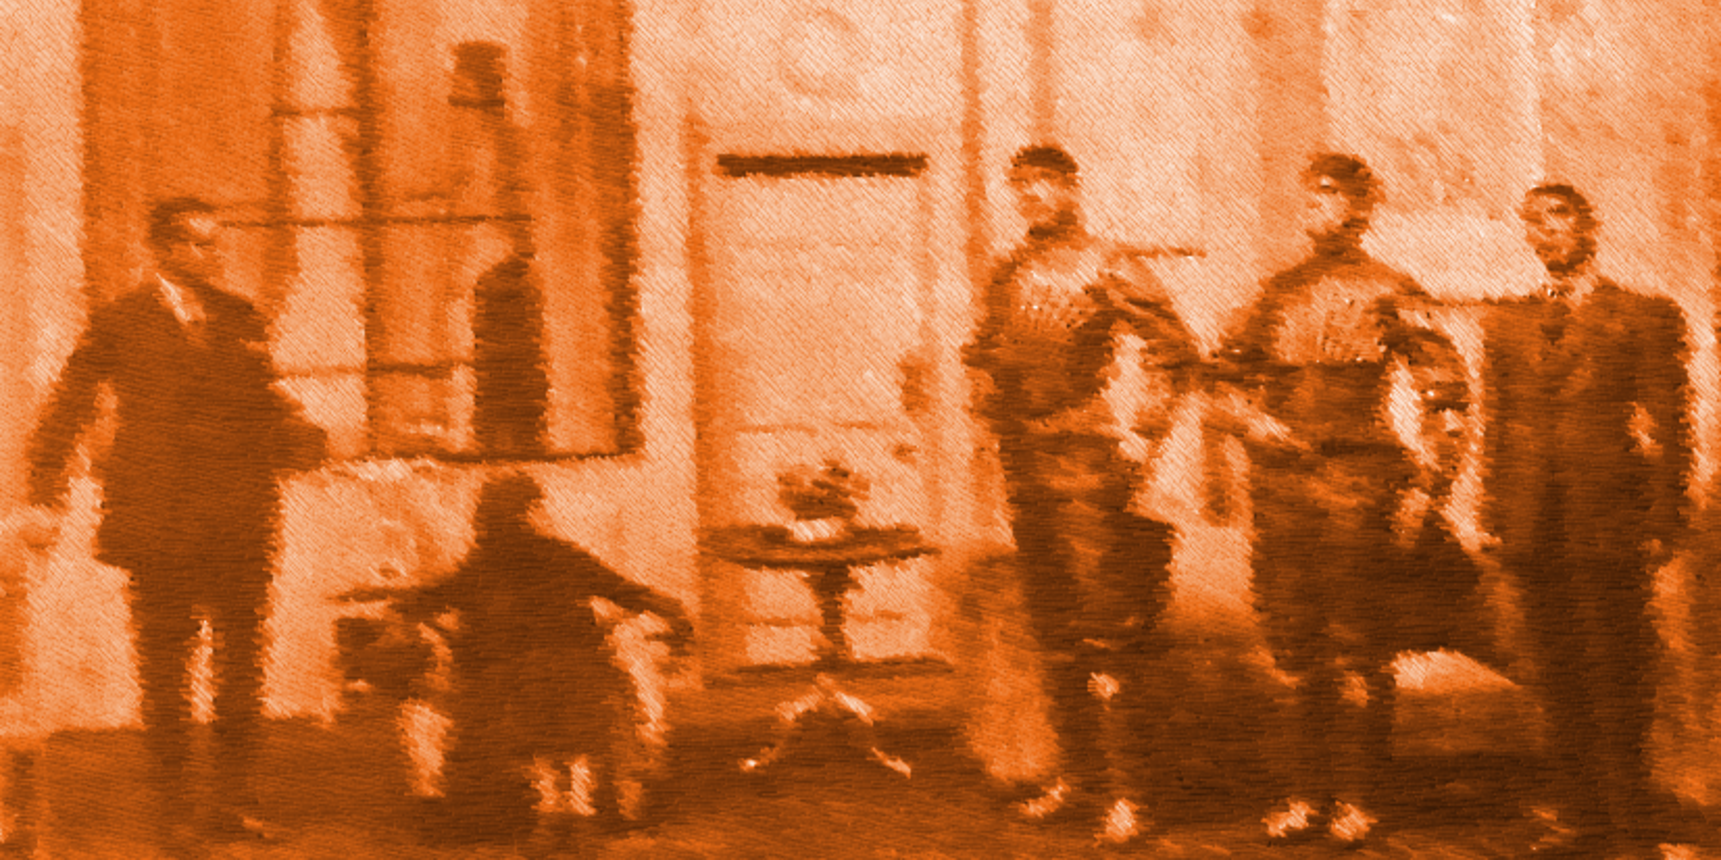
\includegraphics[width=0.30\textwidth]{Capek_play.pdf}
\end{wrapfigure}

R.U.R. (Rossum Universal Robots) was a highly successful science fiction play written by the Czech Karel Čapek in 1920. The play introduced for the first time the word 'robot' as an alternative to other words used at that time like 'automaton' or 'android'. The word 'robot' derives from the Czech 'robota' meaning "forced labor of the kind that serfs had to perform on their masters' lands". The drama occurs in R.U.R., a factory that makes intelligent robots from artificial flesh and bones, so perfect that they can be mistaken for humans (the name Rossum is derived from the Czech word 'rozum' that means 'reason'). At the beginning robots were happy to work for humans, but then a rebellion starts and all the humans are murdered. At the end of the plot, robots realize that they do not have the knowledge to make new robots, and that by exterminating humans they have triggered their own extinction. The play is considered as a tragic satire about a naive humankind, the dangers of technology, and the obsolescence of God.

\subsection* {Wikipedia Monument}

\begin{wrapfigure}{L}{0.3\textwidth}
\centering
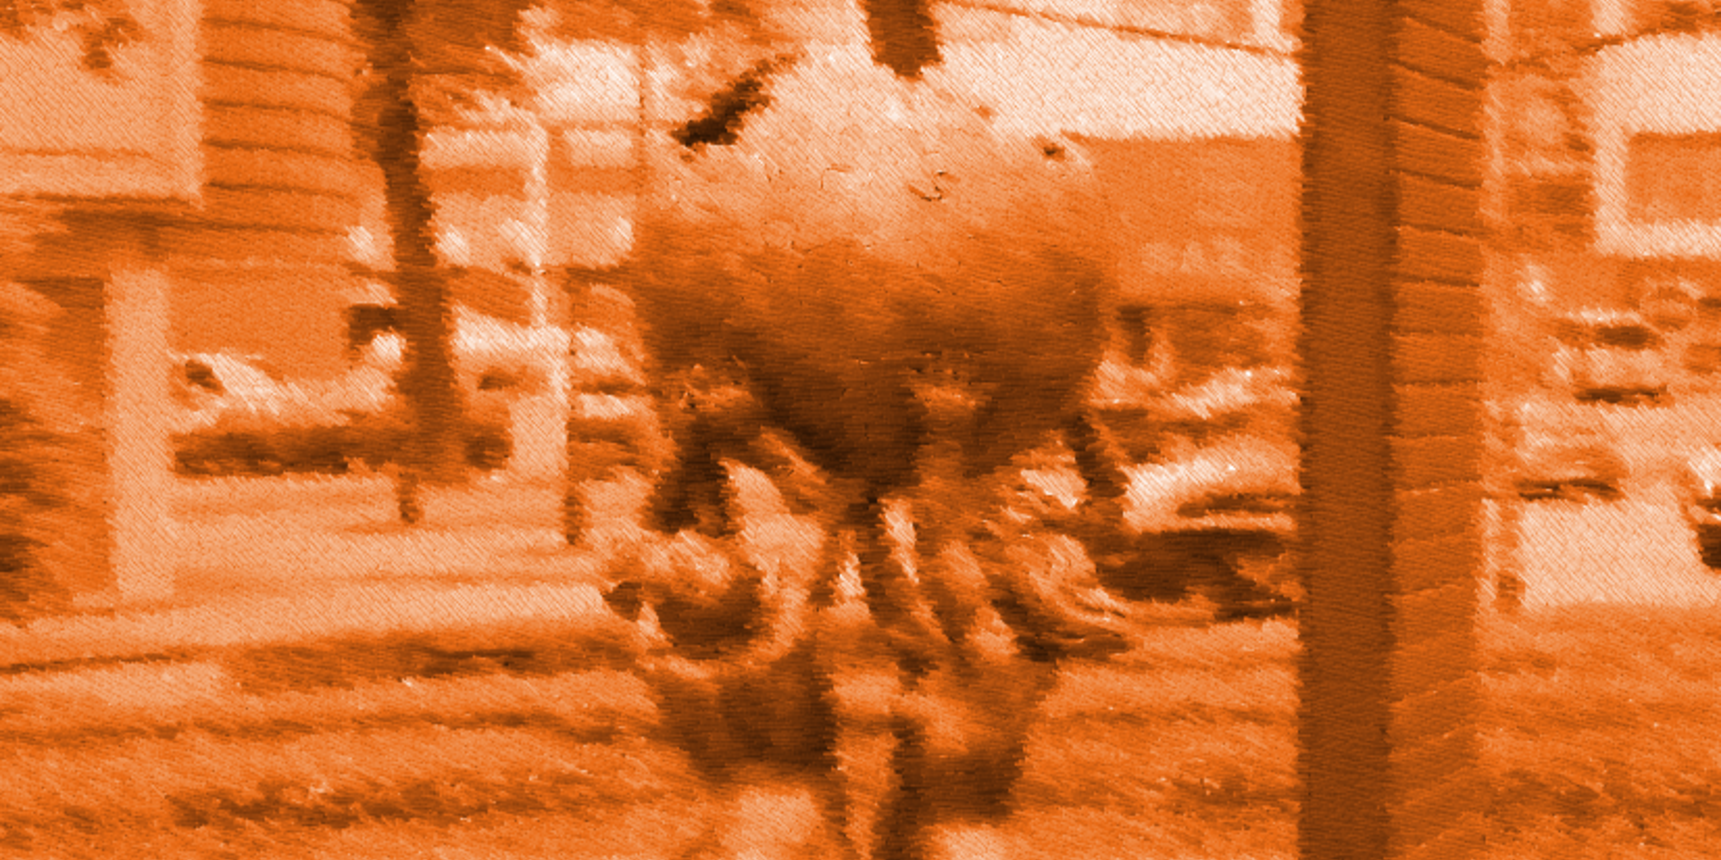
\includegraphics[width=0.30\textwidth]{Wikipedia_Monument_2.pdf}
\end{wrapfigure}

The Wikipedia Monument is located in the city of Słubice, Poland. The statue was designed by Armenian sculptor Mihran Hakobyan, and it was unveiled on October 2014, becoming the world's first monument to the online encyclopedia. The inscription reads: "With this monument the citizens of Słubice would like to pay homage to thousands of anonymous editors all over the world, who have contributed voluntarily to the creation of Wikipedia, the greatest project co-created by people regardless of political, religious or cultural borders. In the year this monument is unveiled Wikipedia is available in more than 280 languages and contains about 30 million articles. The benefactors behind this monument feel certain that with Wikipedia as one of its pillars the knowledge society will be able to contribute to the sustainable development of our civilization, social justice and peace among nations."

